\documentclass[tikz,border=6pt]{standalone}
\usepackage[T1]{fontenc}
\usepackage{lmodern}
\usepackage{amsmath,amssymb}
\usetikzlibrary{positioning,arrows.meta,fit,calc}
% Design of koblitz-n83-closure-indexlift-rep-20261020 (frozen protocol.json and schedule.json). Not a result.
\begin{document}
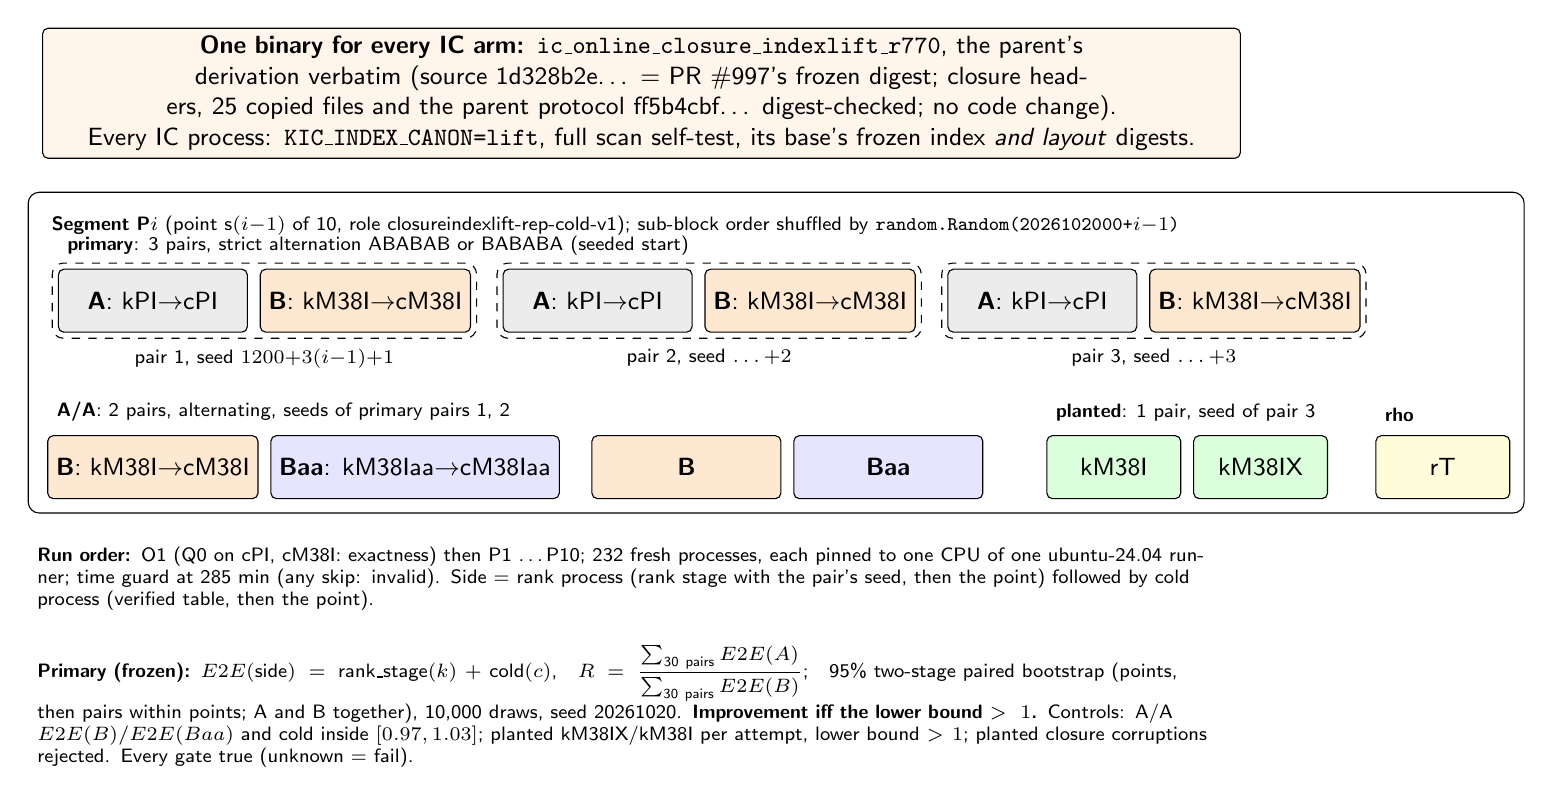
\begin{tikzpicture}[
  font=\sffamily\small,
  box/.style={draw, rounded corners=2pt, align=center, minimum height=8mm, inner sep=3pt},
  sa/.style={box, fill=gray!15, minimum width=24mm},
  sb/.style={box, fill=orange!18, minimum width=24mm},
  sc/.style={box, fill=blue!10, minimum width=24mm},
  sx/.style={box, fill=green!14, minimum width=17mm},
  arr/.style={-{Stealth[length=2.2mm]}, thick},
  note/.style={align=left, font=\sffamily\scriptsize}
]
% producer
\node[box, fill=orange!8, text width=150mm] (prod) {\textbf{One binary for every IC arm:} \texttt{ic\_online\_closure\_indexlift\_r770}, the parent's derivation verbatim
(source 1d328b2e\ldots\ = PR \#997's frozen digest; closure headers, 25 copied files and the parent protocol ff5b4cbf\ldots\ digest-checked; no code change).\\
Every IC process: \texttt{KIC\_INDEX\_CANON=lift}, full scan self-test, its base's frozen index \emph{and layout} digests.};
% one point segment
\node[note, below=6mm of prod.south west, anchor=north west] (ptitle) {\textbf{Segment P$i$} (point s$(i{-}1)$ of 10, role closureindexlift-rep-cold-v1); sub-block order shuffled by \texttt{random.Random(2026102000+$i{-}1$)}};
% primary block
\node[sa, below=3mm of ptitle.south west, anchor=north west, xshift=2mm] (a1) {\textbf{A}: kPI$\to$cPI};
\node[sb, right=1.5mm of a1] (b1) {\textbf{B}: kM38I$\to$cM38I};
\node[sa, right=4mm of b1] (a2) {\textbf{A}: kPI$\to$cPI};
\node[sb, right=1.5mm of a2] (b2) {\textbf{B}: kM38I$\to$cM38I};
\node[sa, right=4mm of b2] (a3) {\textbf{A}: kPI$\to$cPI};
\node[sb, right=1.5mm of a3] (b3) {\textbf{B}: kM38I$\to$cM38I};
\node[draw, dashed, rounded corners, fit=(a1) (b1), inner sep=2pt, label={[note]below:pair 1, seed $1200{+}3(i{-}1){+}1$}] {};
\node[draw, dashed, rounded corners, fit=(a2) (b2), inner sep=2pt, label={[note]below:pair 2, seed $\ldots{+}2$}] {};
\node[draw, dashed, rounded corners, fit=(a3) (b3), inner sep=2pt, label={[note]below:pair 3, seed $\ldots{+}3$}] {};
\node[note, above=0.5mm of a1.north west, anchor=south west] {\textbf{primary}: 3 pairs, strict alternation ABABAB or BABABA (seeded start)};
% aa block
\node[sb, below=13mm of a1] (aa1) {\textbf{B}: kM38I$\to$cM38I};
\node[sc, right=1.5mm of aa1] (aa2) {\textbf{Baa}: kM38Iaa$\to$cM38Iaa};
\node[sb, right=4mm of aa2] (aa3) {\textbf{B}};
\node[sc, right=1.5mm of aa3] (aa4) {\textbf{Baa}};
\node[note, above=0.5mm of aa1.north west, anchor=south west] {\textbf{A/A}: 2 pairs, alternating, seeds of primary pairs 1, 2};
% planted
\node[sx, right=8mm of aa4] (p1) {kM38I};
\node[sx, right=1.5mm of p1] (p2) {kM38IX};
\node[note, above=0.5mm of p1.north west, anchor=south west] {\textbf{planted}: 1 pair, seed of pair 3};
\node[sx, right=6mm of p2, fill=yellow!15] (rt) {rT};
\node[note, above=0.5mm of rt.north west, anchor=south west] {\textbf{rho}};
\node[draw, rounded corners, fit=(ptitle) (a1) (b3) (aa1) (rt), inner sep=5pt] (seg) {};
\node[note, below=3mm of seg.south west, anchor=north west, text width=150mm] (order) {\textbf{Run order:} O1 (Q0 on cPI, cM38I: exactness) then P1 \ldots P10; 232 fresh processes, each pinned to one CPU of one ubuntu-24.04 runner; time guard at 285 min (any skip: invalid).
Side = rank process (rank stage with the pair's seed, then the point) followed by cold process (verified table, then the point).};
\node[note, below=2mm of order.south west, anchor=north west, text width=150mm] (prim) {\textbf{Primary (frozen):}
$E2E(\text{side}) = \text{rank\_stage}(k) + \text{cold}(c)$,\quad
$R=\dfrac{\sum_{\text{30 pairs}} E2E(A)}{\sum_{\text{30 pairs}} E2E(B)}$;\quad
95\% two-stage paired bootstrap (points, then pairs within points; A and B together), 10{,}000 draws, seed 20261020.
\textbf{Improvement iff the lower bound $>1$.} Controls: A/A $E2E(B)/E2E(Baa)$ and cold inside $[0.97,1.03]$; planted kM38IX/kM38I per attempt, lower bound $>1$; planted closure corruptions rejected. Every gate true (unknown = fail).};
\end{tikzpicture}
\end{document}
